\documentclass[jou,apacite]{apa6}
\usepackage{listings}
\renewcommand{\baselinestretch}{1.5}
\setlength{\parindent}{2em}
\setlength{\parskip}{0.5em}

\title{Contemporary Approaches for AI Governance \par in Financial Institutions}
\shorttitle{APA style}

\author{Björn Preuß*}
\affiliation{*Copenhagen Business School, Department of Economics, Government and Business\par
*Copenhagen Business School, Center of Corporate Governance}

\abstract{Organizations want to leverage AI systems by effective use of their data and reduction of risk espoused throughout the operation of AI systems. Given the aim for risk reduction, we see the need for highlighting several AI governance areas. In the paper we explore risks and limits connected with the application of AI models in financial modeling and its application in practice. We will present approaches to overcome limitations and potential biases. Based on an example model, we highlight certain issues and problems. We review current policies and present their requirements. Finally, we discuss how many policies are aligned with the technical possibilities and limits and based on that develop suggestions for changes.\par
Keywords: \textit{AI, Governance, Regulation, Modeling, Machine-Learning, Business}}

\rightheader{NFaGS II Research Project}
\leftheader{NFaGS II Research Project}

\begin{document}

\maketitle    
                        
\section{1. Relevance of regulatory mechanisms on AI models}

AI refers to a statistical system that learns from data samples. Applications to generate value for businesses such as ~\cite{jiang2019prediction} could lead to additional issues with similar complexity that have to be solved.
The need to keep up with management of regulation could lead to the use of technology to do so (e.g. fraud detection); But using technology in a corporate setup for e.g. risk rating might open for new regulatory needs and governance around it. However, only 5-10 percent of executives see a financial gain from applying AI techniques ~\cite{ransbotham2019winning}. See in fact a development for frameworks, guidelines etc. which have to be managed and met by technological solutions in the industry. But having an increasing number of regulations and tooling makes it difficult to identify which governance mechanisms are appropriate and which not. Before deciding which regulations might be suitable, one has to remember what makes an AI system. An AI system is: a) Applicable by having a comparative low cost. Expert systems with similar performance have a significantly higher cost. b) AI systems have a higher complexity. Hence this it is much more difficult to understand how they work. Determine how an AI system decided is often difficult for people to define. c) With the complexity in mind, it is straightforward to understand that AI systems are often outside of the control of an organization. Applying statistical techniques result often in unexpected outcomes. Data issues such as biases might also affect the model’s outcome ~\cite{morgulis2019fooling}. d) The speed at which AI systems and with that opportunities are developing creates significant pressure on regulations to keep up ~\cite{cihon2019standards}.\par

To work with systems having such features, one has to design governance mechanisms fitting it. We can define regulation of it systems as rules, practices and processes to direct and control AI ~\cite{almeida2020artificial}~\cite{winfield2019machine}. It covers the fields of used data, the modeling approach and the explainability of the model and responsibilities and general security. The development of systems using AI models or models based on machine learning and or deep learning require an update of the current regulatory landscape. This is more true, hence e regulation often focuses on preventing harm rather than leveraging AI capabilities ~\cite{winfield2019machine}. This holds especially true when those models should be applied in industries or functions which have traditionally a high regulatory standard. This is, for example, the financial industry.\par
 
Building on this motivation, the paper aims to give a transparent view on the literature and the legal frameworks around it. By showing technical limitations and possibilities at an example, we will point towards gaps which regulators should focus at. after doing so, we will enter the discussion towards regulatory approaches around predictive models in the financial sector. We will cover current approaches and highlight how one could adapt these with having technological possibilities in mind and without stopping the development of advanced models in finance. Alongside the discussion of the literature, the technical capabilities of today’s systems will be highlighted shortly to give the reader a perspective on what is possible. Based on the study of the literature and the modeling demo, we aim to find gaps or misalignment in the literature which can be used to discuss topics at a level of policy makers.\par

We will review the contemporary literature on the topic to define developments and the status of governance of AI. We will discuss furthermore the applicability of frameworks and ask for practicality. This will lead to suggestions of change to regulations which are currently possible to implement in practice from a technical point of view.

\section{2. Regulation of Applied Statistical Models}

Before going into detail reviewing mechanisms, we have to define what we mean by AI governance. One can define AI governance as \textit{Processes, structure, practices and rules that ensure the organization’s strategy and objectives.} We align in our definition with views of ~\cite{abraham2019data} by highlighting certain functions such as formalizing AI management, focusing on AI as part of strategy, developing policies, standards and procedures and monitoring compliance’s. At this point we want to further introduce the view of AI system as being not only the model but the data, the model and the system (components around it) that have to be governed ~\cite{schn19}.\par

We can see governing of AI systems as formal structures connecting business, data model and IT system management ~\cite{schn19} ~\cite{peterson2004crafting}. We can group the different parts into i) structural, ii) procedural and iii) relational parts see, ~\cite{peterson2004crafting} and ~\cite{van2009enterprise}. With regulation, we see different areas where regulators touch upon machine learning models or artificial intelligence (AI). Splitting them into groups we can refer to the ones introduced by ~\cite{peterson2004crafting}. 

The first and third group being structural and relational mechanisms are quite clear. Under structural mechanisms, one to be mentioned is that current AI systems are in relation to the segregation of duties less developed. The responsibility is not divided by roles which would be from importance. The last group relational mechanisms are important for knowledge sharing and information delivery, but less model specific. The first to name under the second group, being structural mechanisms, is model impact. It is crucial to define the impact that the model will have and to store this information. We see certain areas of application more critical and hence this the models applied more impact-full. Examples of these could be industries such as healthcare, education or finance ~\cite{angwin2016machine} ~\cite{mitchell2019model}. \par

With high impact models, it is even more crucial to select the best in class models for a problem. Also, one has to document the selection process that when an issue arises, one can go back and see why a model was selected. The literature suggests for this benchmark approaches and systems that store the benchmark options immutable ~\cite{gebru2018datasheets}. Such systems exist already in regulated industries which uses quantitative models to support decisions such as the financial industry, e.g. credit rating. For being able to benchmark models and to select the best model, one has to not only take the model’s performance, such as accuracy or f1 score into consideration, but also the “reasoning” which the model uses. For this a framework called XAI for explainable AI was developed and is until now still under development~\cite{adadi2018peeking} ~\cite{schneider2019personalized} ~\cite{das2020opportunities}. By reasoning, we mean the variables the model uses to predict and the impact that these variables play in the model. ~\cite{goodman2017european} suggests in his paper that model explainability  is a key component in the EU law on model explainability. The explainability is a corner stone when applying machine learning to high-risk areas such as finance. If models such as neural networks (see here the application of RNN LSTM) can not supply explainability then we have to exclude them from a possible model selection. ~\cite{goodman2017european}

Options such as saliency maps, TCAV ~\cite{kim2018interpretability} allow to explain how neural networks on for example images work. Concept activation vectors (TCAV) work in the way that it uses directional derivatives to quantify which concept is important to a classification result–for example, how sensitive a prediction of “car-damage” is to the presence of "unformed parts". An other approach trying to explain image recognition is the GradCam framework which we do not want to discuss further but which we want to name\footnote{GradCam shows the activation of the network used for image classification as a heat-map. With this the user can explore which features made the model do a specific decision. The python package can be found on github}. 
An other option are path integrated gradients, these aim to assign an importance value to each input feature of a deep-learning or machine learning model based on the gradients of the model output with respect to the input ~\cite{kaushik2018did} ~\cite{sundararajan2017axiomatic}. In simple terms it simulates input parameters and measures, which feature drives the predictions the most.\par

Especially in finance, we see a high risk of model bias. Model bias has to be eliminated. We can state that each model based on variables will have some sort of bias hence it predicts based on statistical structures in the data. But for the application of such a model, there are certain variables which the model should not be biased towards. One example is gender. For antibias or more positively formulated fairness, there are certain methods addressing this on a model level ~\cite{du2020fairness}. As we have seen in the example above, there was to test for variable bias and also to eliminate the bias. The simplest form of bias elimination would actually be to remove the critical variable form the training data-set. Unfortunately, high-risk variables often contain quite some useful information and they often make sense. E.g. a 18-year-old guy with a golf GTI will usually drive faster, hence that he should be priced higher in his insurance. That fact and the pricing are widely accepted. However, this does not mean that every male person has to be priced higher. Besides the approaches shown in the code above, there are libraries that can detect model bias and store the information one example for this is the cards highlighting of model behavior from ~\cite{mitchell2019model}. On the application side model bias has let to problems not only in financial applications. However, one has to know that until now what fairness means is not until the end defined and still a point of discussion ~\cite{verma2018fairness}. But there are some characteristics that research and authorities align and which they define as to be protected, such as religion, gender as ~\cite{corbett2018measure}. One highly critical example could be medical trials. When they are run on men, they could lead to problems when applying results on women as shown by ~\cite{westervelt2015medical}. \par

Besides the actual model, there is more to monitor. This is the actual work with such model, who has worked on them and who has deployed them etc.. Here AI specific regulation meets traditional it regulation frameworks such as data privacy (GDPR) ~\cite{tankard2016gdpr}. 

With machine learning we not only have to know how good a model is and why the model does a prediction but also who has worked with it and when was the model deployed, which data was used etc. Policies as those published from ~\cite{goodman2017european} might be a starting point but from and organizational perspective ~\cite{alsheiabni2020winning} suggest using best practices for internal policies. That does not mean that existing policies are accepted across academics. Scholars such as ~\cite{mishra2020measurement} might not with all align. But in fact the possibility for reproduction and the ability to manage models etc. comes with various challenges touching upon the data, model, concept, management and engineering level ~\cite{schelter2018automating} ~\cite{schn19}. This quest need to lead to systems supporting modelings and the management of models, but also coding guidelines ~\cite{stoica2017berkeley} and data. \par

Data is besides the model, the most sensitive piece of a machine learning system. The standards related to data have been widely developed~\cite{mosley2010dama}. Data and the use of data is especially in Europe highly regulated and especially for certain industries as pharmacy or the public sector there are limits. Hence this, ~\cite{gebru2018datasheets} asks for a standard way of documentation of data and data usage ~\cite{bender2018data}. The development of AI standards similar to data standards is currently ongoing, see for this ~\cite{cihon2019standards}. For machine learning applications, one part where data also affects the functioning of the model is the selection of the training data. The training data should match the data in production and so have also the test data fit the reality. If one has mainly young people as a customer and wants to rate them, then it makes little sense if one trains a model on old aged people with potentially other characteristics (age, employment, savings, etc.) ~\cite{gebru2018datasheets}.\par

Especially in highly regulated industries, we see a faster adoption of such regulations. These industries are historically the first that are asked to be compliant, and often this goes hand in hand with a higher level of risk and impact on the society. This leads to the importance of data management and documentation not only on the model level ~\cite{garvie2016perpetual} ~\cite{mann2016hiring}. But despite this, right now there is no standard way of documentation of data that is used in machine learning ~\cite{thelisson2017regulatory}. In fact, often the processes use data and methods to transform the data and then it enters a black box that no one fully oversees which creates an even bigger problem than just poor documentation ~\cite{gebru2018datasheets}. It creates the risk of huge mistakes hence the work can not be checked.\par


\section{3. Method}

Building on the review of contemporary studies. We use add to the literature not only by a comprehensive review but also by an experiment to show gaps and limitations in the current understanding of AI governance. \par

We use secondary data to determine the need of regulations. We showcase this need also in a code example on simulated transaction data.  The case will try to predict fraudulent transactions in the simulated transaction data. We generate the data with the PaySim simulation engine. For the demonstration of certain problems, we train a recurrent neural network (RNN) implementing a Long short-term memory (LSTM) model. We can obtain the formal description from the formula (1) to (6).\par

$f_t = \sigma_g (W_f x_t+U_f h_t+b_f)$ (1)\par
$i_t = \sigma_g (W_i x_t+U_i h_t+b_i)$ (4)\par
$o_t = \sigma_g (W_o x_t+U_o h_t+b_o)$ (3)\par
$\tilde{c}_t = \sigma_g (W_c x_t+U_c h_t+b_c)$ (4)\par
$c_t=f_t^o c_{t-1}+i_t^o\tilde{c}_t$ (5)\par
$h_t=o_t^o\sigma_h(c_t)$ (6)\par

The formulas describe the theoretical notion of the used LSTM model where the initial values are  $c_{0}=0$ $c_{0}=0$ and $h_{0}=0$ $h_{0}=0$ and the operator  denotes the Hadamard product (element-wise product). The subscript $t$ indexes the time step. It furthermore used the following variables:\par

${\displaystyle x_{t}\in \mathbb {R} ^{d}}$: input vector to the LSTM unit \\
${\displaystyle f_{t}\in \mathbb {R} ^{h}} {\displaystyle f_{t}\in \mathbb {R} ^{h}}$: forget gate's activation vector \\
${\displaystyle i_{t}\in \mathbb {R} ^{h}} {\displaystyle i_{t}\in \mathbb {R} ^{h}}$: input/update gate's activation vector \\
${\displaystyle o_{t}\in \mathbb {R} ^{h}} {\displaystyle o_{t}\in \mathbb {R} ^{h}}$: output gate's activation vector \\
${\displaystyle h_{t}\in \mathbb {R} ^{h}} {\displaystyle h_{t}\in \mathbb {R} ^{h}}$: hidden state vector also known as output vector of the LSTM unit \\
${\displaystyle {\tilde {c}}_{t}\in \mathbb {R} ^{h}} {\displaystyle {\tilde {c}}_{t}\in \mathbb {R} ^{h}}$: cell input activation vector \\
${\displaystyle c_{t}\in \mathbb {R} ^{h}} {\displaystyle c_{t}\in \mathbb {R} ^{h}}$: cell state vector \\
${\displaystyle W\in \mathbb {R} ^{h\times d}} {\displaystyle W\in \mathbb {R} ^{h\times d}}, {\displaystyle U\in \mathbb {R} ^{h\times h}} {\displaystyle U\in \mathbb {R} ^{h\times h}} and {\displaystyle b\in \mathbb {R} ^{h}} {\displaystyle b\in \mathbb {R} ^{h}}$: weight matrices and bias vector parameters which need to be learned during training \par

We train the model in a supervised fashion where we will tell the model which of the transactions has been fraudulent and which not. Before training we will align the classes hence we deal with an imbalance data-set. Starting from this, we will show which options for measuring model impact and how to get model transparency. This showcase will enable us to leave room for a discussion on whether certain regulations should be adjusted and if so how. We will also give a hint towards further technical development which try to overcome challenges we see today in measuring bias or getting model transparency.

\section{4. Modeling Issues and Technical Capabilities}

Before starting the discussion around different areas of regulation, we have to look at technical capabilities. Some proposed regulatory steps are limited by the technical capabilities. That, of course, does not mean that we will see a development from a technical perspective, but opportunities need to be viewed. With this we aim in this chapter to highlight the actual capabilities plus show some angles for further development of approaches.\par

I would like to start with issues arising from the development of models and problems that are directly linked to the mathematics of the model. For this we have constructed an example model based on simulated payment transactions, which include fraudulent transactions. On top of the data, we trained a model aiming to detect the fraud-transactions. The used data-set includes the following variables from which some are categorical, the rest are numeric:

\begin{lstlisting}[language=Python]
columns = ["step*",
"type*",
"amount",
"nameOrig*",
"oldbalanceOrg",
"newbalanceOrig",
"nameDest*",
"oldbalanceDest",
"newbalanceDest",
"isFraud*",
"sex*",
"age"]
\end{lstlisting}

The columns marked with a * are categorical columns, the ones without are numeric. A critical feature is the variable gender. One central element of the procedural mechanism was the measurement of bias and the impact of it on the modeling result. Here one has to run some tests to insure a non-bias of the data and later the model. Usually we can say that most model bias comes from bias in the data. Usually one can identify high-risk variables for which one should run tests for bias, as we will show here for the variable gender as mentioned in the literature before. In the following plot one can see that gender is balanced in the data-set. See figure: ~\ref{sch:gender}.

\begin{figure}[htb!]
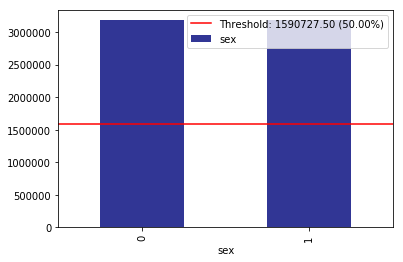
\includegraphics[width=8cm, height=5cm]{genderbalance.png}
\caption{: Gender balance in the data set}
\medskip % induce some separation between caption and explanatory material
\begin{minipage}{0.45\textwidth} % choose width suitably
{\footnotesize Note: The figure shows that both gender (male and female) are same often in the data. We do not see a situation on imbalanced features.\par}
\end{minipage}
\label{sch:gender}
\end{figure}

When we include the fraud class (data label) of a transaction we see, however, that we have an imbalanced situation. This is partly because we have less fraud transaction than clean ones and that in the data, the gender variable is not normally distributed among fraud and non-fraud. Meaning we can see that more male have fraud transactions. This in-balance might lead to a gender bias in a later prediction model, see figure: ~\ref{sch:genderim}.

\begin{figure}[htb!]
  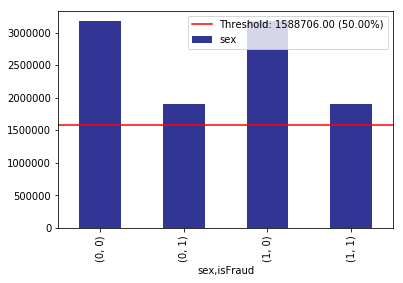
\includegraphics[width=8cm, height=5cm]{rebalancegenderfraud.png}
  \caption{: Gender / Fraud imbalance}
  \medskip % induce some separation between caption and explanatory material
  \begin{minipage}{0.45\textwidth} % choose width suitably
  {\footnotesize Note: After introducing the classes however, we see a different  picture. By plotting the classes divided by the risk variable gender, we see an im-balanced picture.\par}
  \end{minipage}
  \label{sch:genderim}
\end{figure}

It is critical to mention that there will always be certain correlations in the data-set and hence this biases. However, it is important that we limit the biases for high-risk variables as much as possible to avoid certain conflicts with societal interest. We do not want a model that discriminates a man over a woman or vice versa. When identifying such a situation, one can use statistical approaches to even out this imbalanced situation so that the gender is same often represented in fraudulent transactions. See for this Appendix I.\par

Besides looking for high-risk variables, we could suggest starting with looking at correlated variables. This approach would be neutral and data driven and hence this could be automated, for example in an auto-ml setup. Here one can suggest a classical correlation matrix as shown in the following figure: ~\ref{sch:corre}.

\begin{figure}[htb!]
  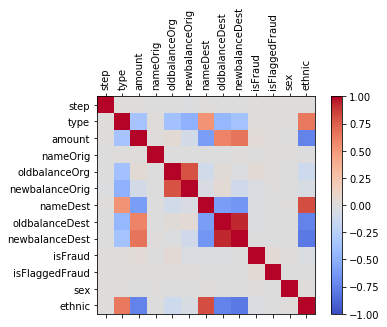
\includegraphics[width=8cm, height=7cm]{correlation.png}
  \caption{: Correlation matrix heat-map}
    \medskip % induce some separation between caption and explanatory material
        \begin{minipage}{0.45\textwidth} % choose width suitably
        {\footnotesize Note: The heat-map shows the correlation of variables in the data. The darker (more red) the color is the higher the correlation between the features..\par}
        \end{minipage}
  \label{sch:corre}
\end{figure}

After identifying features from this it is possible to eliminate bias as with the gender example, or if possible eliminate features that are unnecessary. In our case, we do not define such features so we can go on with the training of the LSTM model. The code for this we have described in Appendix II.\par

After training the model we can measure the performance and also split the performance of the train test split by gender or any other high-risk variable we are interested in. We do this by using the framework of XAI which we referred to in the literature. We do this with the variable gender in figure: ~\ref{sch:perform}.

\begin{figure}[]
  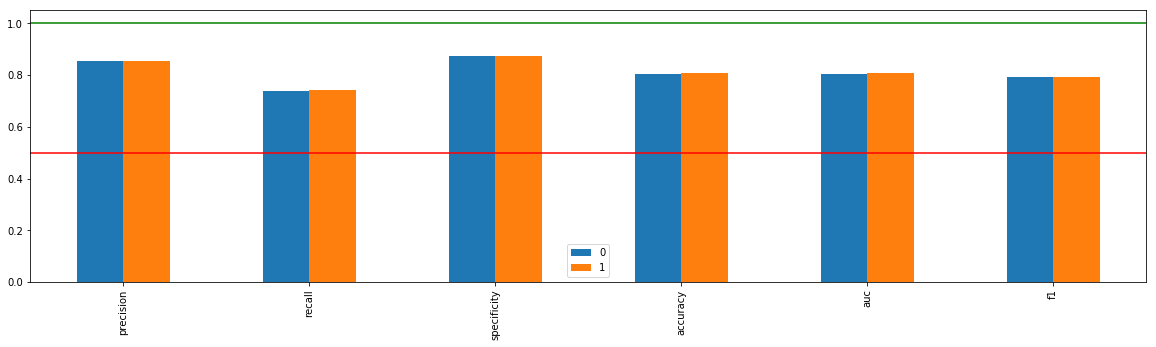
\includegraphics[angle=90, width=8cm, height=20cm]{genderperformancesplit.png}
  \caption{: Performance metrics comparison by gender}
    \medskip % induce some separation between caption and explanatory material
    \begin{minipage}{0.45\textwidth} % choose width suitably
    {\footnotesize Note: The plot shows that after following the guide, there is no difference in the model performance per gender.\par}
    \end{minipage}
  \label{sch:perform}
\end{figure}

The graph shows that after the even out of the variable we see no bias in the performance metrics of the LSTM model for gender. With this we have eliminated potential gender bias in the data and with this in the model. \par

The second point which is crucial is model explainability. Especially for non-linear model like the here used LSTM model, we have to search for ways to get a variable or feature importance. Classical probabilistic models have the option to get these directly. With non-probabilistic models one has to use other approaches to get with reasonable computation a variable importance that is as close to the reality as possible. We can use here frameworks such as shap \footnote{SHAP (SHapley Additive exPlanations) is a game theoretic approach to explain the output of any machine learning model. It connects optimal credit allocation with local explanations using the classic Shapley values from game theory and their related extensions (see papers for details and citations)}, lime \footnote{Lime is able to explain any black box classifier, with two or more classes. All we require is that the classifier implements a function that takes in raw text or a numpy array and outputs a probability for each class. Support for scikit-learn classifiers is built-in} or eli5 \footnote{ELI5 is a Python package which helps to debug machine learning classifiers and explain their predictions.}. These frameworks enable the researcher or practitioner building advanced models to keep a level of transparency.\par

Beside these model specific requirements, one can see more environment requirements. Here we leave the model level and look more at the production environment or AI-system that runs such models. Just running a model is not enough. We have to retrace changes in the model through logs and timestamps. Certain systems like GIT frameworks enable the developer to store code versions but often not algorithm versions. Here we might require advanced logging functionality to capture changes in the model over time while it runs in production. Besides logs and version controls, we can also see questionnaires as use full to store relevant information after each model release. This could be an extensive read-me document that is changed after each release, but much better would be a system that can store the answers and log the responses to inform the user about it.\par

We see the AI-system also overtaking functionality like segregation of duties, logging functionality and user access and security related functionality. It enables to run the models in a secure and operators friendly environment and makes with that the deployment of models on scale. Besides procedural mechanisms, the system also covers relational mechanisms such as communication and knowledge sharing. It furthermore also enables some structural mechanism by having an extensive role management.

\section{5. Should we limit Machine Learning in Finance?}

The analysis of possibilities to govern non-linear models in financial applications leads to some discussion points that we want to highlight here. The first one being centered on the model and understanding the model’s performance over its lifetime as well of biases. We see that there is a discrepancy between the frameworks published and the technical capabilities in building non-linear models. Instead of working with technical people together, it seems as regulators have come up with soft requests that are easy to full-fill and without specific recommendations on how to do it. Here the companies will be on their own in thinking how to full-fill the requirements. Based on the presentation of technical possibilities in the beginning of this paper, we suggest an update of regulations with more concrete methods and recommendations. Here I would like to name f.ex. (i) bias metrics or best practices for (ii) measuring model performance and (iii) variable importance. We have to bring an understanding of these techniques into the frameworks to support businesses when fulfilling the regulations. Without that we might see uncontrolled and ineffective developments because of unknown possibilities. Novel approaches and model have different requirements, but naming best practices and aligning regulations with the capabilities would be beneficial.\par

That alignment of regulatory requirements with technical capabilities will not only increase the level of concreteness but also enforce stricter but doable regulation on to businesses. This might help the regulator reach its goals more than with the soft frameworks available today. If it is possible for companies to be compliant, then we will also see more AI models being developed with the regulations in mind. If we fail in having strict but achievable guidelines, we will either see models not comply to regulations or see no models being developed, so European organizations might have some risk to not be competitive.\par

The second area we would like to discuss is around the process of model deployment and production of models. Reviewing current ethical guidelines and regulations, we see many quests related to the way of how models are made. Regulations are not only related to the data and the models with its potentially inherited biases, it is also focused on the system managing the AI models. This in our eyes creates a risk that it burdens the technical development with a manual on paper regulation. Here, as with the model performance, we have to ask what technical capabilities exist to full-fill regulations without increasing manual regulations. Tracking of actions on the models and process regulations should be enforced technically in a system. procedural mechanism that work with technical tracking and other side AI-systems that have beside functional requirements also regulations as a basis will be the way to go. We should not cover regulations with manual on paper regulation hence this would slow down development and lower the competitiveness of organizations falling under these regulations. Instead, one should bring the performance tracking and action logging together to allow for a big-picture view on the model and the model life cycle.\par

The mentioned structural mechanisms should be supplemented by the technical system but should mostly be enforced by established governance mechanisms such as the board of directors on the high level and other control mechanisms such as data-audits and laws on an operative level.


\bibliography{sample}

\section{Appendix}

\subsection{I Compliance with Ethical Standards}
\textit{Conflict of Interest:} The authors declare that they have no conflict of
interest.\par
\textit{Ethical Approval:} All procedures performed in studies involving human
participants were in accordance with the ethical standards of the institutional
and/or national research committee and with the 1964 Helsinki
declaration and its later amendments or comparable ethical standards.
This article does not contain any studies with animals performed by
any of the authors.\par
\textit{Informed Consent:} Informed consent was obtained from all individual
participants included in the study.

\subsection{II Even out Variable Bias}
With the following code we even out bias in the data. This is done by having same examples of each gender with fraud and clean transactions.\par

\begin{lstlisting}[language=Python]
proc_df = bal_df #xai.normalize_numeric
(bal_df)
proc_df = xai.convert_categories
(proc_df)
x = proc_df.drop("isFraud", axis=1)
y = proc_df["isFraud"]

x_train, y_train, x_test, y_test, 
train_idx, test_idx = 
\xai.balanced_train_test_split(
        x, y, "sex", 
        min_per_group=8000,
        max_per_group=8000,
        categorical_cols=
        categorical_cols)

x_train_display = bal_df[train_idx]
x_test_display = bal_df[test_idx]

print("Total number of examples:", 
x_test.shape[0])

df_test = x_test_display.copy()
df_test["isFraud"] = y_test

_= xai.imbalance_plot(df_test, 
"sex", "isFraud", categorical_cols=
categorical_cols)
\end{lstlisting}

\subsection{III Training the LSTM Model}
Here we describe the code used for training the LSTM model. Further docusmnetation can be obtained from the notebook.\par

\begin{lstlisting}[language=Python]
import sklearn
from sklearn.model_selection 
import train_test_split
from sklearn.metrics 
import classification_report, 
mean_squared_error, roc_curve, auc

from keras.layers import Input, 
Dense, Flatten, 
\Concatenate, concatenate, 
Dropout, Lambda
from keras.models import Model, 
Sequential
from keras.layers.embeddings 
import Embedding

def build_model(X):
    input_els = []
    encoded_els = []
    dtypes = list(zip(X.dtypes.index, 
    map(str, X.dtypes)))
    for k,dtype in dtypes:
        input_els.append(Input(shape=
        (1,)))
        if dtype == "int8":
            e = Flatten()(Embedding
            (X[k].max()+10, 1)(input_els[1]))
        else:
            e = input_els[0]
        encoded_els.append(e)
    encoded_els = concatenate(encoded_els)

    layer1 = Dropout(0.5)(Dense(100, 
    activation="relu")(encoded_els))
    layer2 = Dropout(0.5)(Dense(300, 
    activation="relu")(encoded_els))
    layer3 = Dropout(0.5)(Dense(400, 
    activation="relu")(encoded_els))
    layer4 = Dropout(0.5)(Dense(300, 
    activation="relu")(encoded_els))
    layer5 = Dropout(0.5)(Dense(100, 
    activation="relu")(encoded_els))
    out = Dense(1, activation='sigmoid')
    (layer1)

    # train model
    model = Model(inputs=input_els, 
    outputs=[out])
    model.compile(optimizer="adam", 
    loss='binary_crossentropy', 
    metrics=['accuracy'])
    return model


def f_in(X, m=None):
    """Preprocess input so it 
    can be provided"""
    if m:
        return [X.iloc[:m,i] for i 
        in range(X.shape[1])]
    else:
        return [X.iloc[:,i] for i 
        in range(X.shape[1])]

def f_out(probs, threshold=0.5):
    """Convert probabilities 
    into classes"""
    return list((probs >= threshold)
    .astype(int).T[0])
\end{lstlisting}

\end{document}
